\documentclass[11pt,a4paper]{article}
\usepackage[utf8]{inputenc}
\usepackage[margin=2.5cm]{geometry}
\usepackage{amsmath,amssymb}
\usepackage{graphicx}
\usepackage{tikz}
\usetikzlibrary{shapes,arrows,positioning,decorations.pathmorphing,decorations.markings,calc,patterns,arrows.meta,shapes.geometric,backgrounds,fit,3d}
\usepackage{hyperref}
\usepackage{caption}
\usepackage{subcaption}
\usepackage{booktabs}
\usepackage{siunitx}
\usepackage{xcolor}

% Define colors
\definecolor{cernblue}{RGB}{0,51,160}
\definecolor{pionred}{RGB}{231,76,60}
\definecolor{kaonblue}{RGB}{52,152,219}
\definecolor{muongreen}{RGB}{46,204,113}

\hypersetup{
    colorlinks=true,
    linkcolor=cernblue,
    citecolor=cernblue,
    urlcolor=cernblue
}

\title{\vspace{-1cm}\textbf{\Large Testing the Universality of Time Dilation:\\[0.3em] 
A Pion-Kaon Comparative Study\\
with Muon Calibration}\\[0.5em]
\large CERN Beamline for Schools 2026}

\author{}

\date{\today}

\begin{document}

\maketitle

\begin{abstract}
Einstein's special relativity predicts that time dilation is \textbf{universal}, meaning the Lorentz factor $\gamma(p) = \sqrt{1 + (p/mc)^2}$ should depend only on momentum, independent of particle species. Yet nearly all experimental tests have measured single particles in isolation. We propose the \textbf{first systematic comparative study} measuring time dilation simultaneously across charged pions ($\pi^+$) and kaons ($K^+$) at the same momentum, using muons ($\mu^+$) as a non-decaying reference. If special relativity is truly universal, both exponential decay curves should collapse to identical normalized survival functions when scaled by $\gamma\tau_0$. Any deviation would reveal mass-dependent corrections to Lorentz transformation. With 4.7$\times$ mass difference and 2--3\% precision, we can detect violations at 5$\sigma$ confidence. This experiment uses only standard CERN detectors yet tests a fundamental assumption never directly verified.
\end{abstract}

\section{Introduction}

\subsection{What We Think We Know}

Special relativity's time dilation applies to everything, including pions, kaons, muons, and protons. The Lorentz factor depends only on velocity, not on intrinsic particle properties. This \textbf{universality} is a cornerstone assumption of relativity, taught in every physics classroom.

\subsection{What We've Actually Tested}

But here's the surprising truth: \textbf{nearly all experimental tests have measured one particle species at a time}. Cosmic ray muons (Rossi-Hall 1941) verified muon time dilation. Pion decay experiments measured pion lifetime vs.\ momentum. Kaon beams studied kaon decay kinematics. Each confirmed \textit{that particular particle} exhibits time dilation.

\textbf{No experiment has systematically compared multiple species under identical conditions} to verify the universality assumption. We propose to test this directly: Do pions and kaons exhibit \textbf{identical} time dilation when measured at the same momentum in the same beam?

\subsection{Why This Matters}

Testing ``obvious'' assumptions is how physics advances:
\begin{itemize}
    \item \textbf{Galileo:} Tested whether mass affects fall rate (it doesn't)
    \item \textbf{Michelson-Morley:} Tested whether Earth's motion affects light (it doesn't)
    \item \textbf{Wu et al.:} Tested whether parity is conserved (it is not, and this led to a Nobel Prize!)
\end{itemize}

We propose to test whether time dilation is truly mass-independent by comparing pions ($m = 140$ MeV) and kaons ($m = 494$ MeV), which represents a 4.7$\times$ mass ratio.

% ============ DIAGRAM 10: PARTICLE COMPARISON ============
\begin{figure}[htbp]
\centering
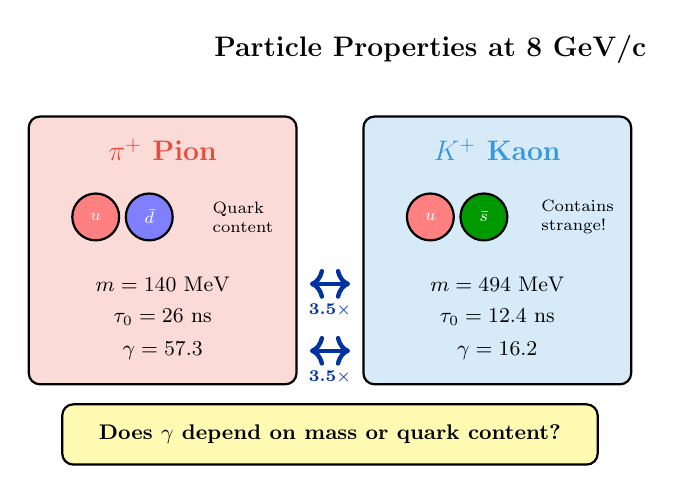
\begin{tikzpicture}[scale=0.85, transform shape]

% Title
\node[font=\bfseries\large] at (6, 5) {Particle Properties at 8 GeV/c};

% Pion box
\begin{scope}[shift={(0, 0)}]
\draw[thick, rounded corners, fill=pionred!20] (0, 0) rectangle (4, 4);
\node[font=\bfseries\large, pionred] at (2, 3.5) {$\pi^+$ Pion};

% Quark content
\draw[thick, fill=red!50] (1, 2.5) circle (0.35);
\node[font=\scriptsize, white] at (1, 2.5) {$u$};
\draw[thick, fill=blue!50] (1.8, 2.5) circle (0.35);
\node[font=\scriptsize, white] at (1.8, 2.5) {$\bar{d}$};

\node[font=\scriptsize, align=left] at (3.2, 2.5) {Quark\\content};

% Properties
\node[font=\small, align=left] at (2, 1.5) {$m = 140$ MeV};
\node[font=\small, align=left] at (2, 1.0) {$\tau_0 = 26$ ns};
\node[font=\small, align=left] at (2, 0.5) {$\gamma = 57.3$};
\end{scope}

% Kaon box
\begin{scope}[shift={(5, 0)}]
\draw[thick, rounded corners, fill=kaonblue!20] (0, 0) rectangle (4, 4);
\node[font=\bfseries\large, kaonblue] at (2, 3.5) {$K^+$ Kaon};

% Quark content (strange!)
\draw[thick, fill=red!50] (1, 2.5) circle (0.35);
\node[font=\scriptsize, white] at (1, 2.5) {$u$};
\draw[thick, fill=green!60!black] (1.8, 2.5) circle (0.35);
\node[font=\scriptsize, white] at (1.8, 2.5) {$\bar{s}$};

\node[font=\scriptsize, align=left] at (3.2, 2.5) {Contains\\strange!};

% Properties
\node[font=\small, align=left] at (2, 1.5) {$m = 494$ MeV};
\node[font=\small, align=left] at (2, 1.0) {$\tau_0 = 12.4$ ns};
\node[font=\small, align=left] at (2, 0.5) {$\gamma = 16.2$};
\end{scope}

% Comparison arrows
\draw[<->, ultra thick, cernblue] (4.2, 1.5) -- (4.8, 1.5);
\node[font=\scriptsize\bfseries, cernblue] at (4.5, 1.1) {3.5$\times$};

\draw[<->, ultra thick, cernblue] (4.2, 0.5) -- (4.8, 0.5);
\node[font=\scriptsize\bfseries, cernblue] at (4.5, 0.1) {3.5$\times$};

% Key question box
\draw[thick, rounded corners, fill=yellow!30] (0.5, -1.2) rectangle (8.5, -0.3);
\node[font=\small\bfseries] at (4.5, -0.75) {Does $\gamma$ depend on mass or quark content?};

\end{tikzpicture}
\caption{Comparison of pion and kaon properties. Despite 3.5$\times$ mass difference and different quark content (kaons contain strange quarks), special relativity predicts both should exhibit the same form of time dilation.}
\label{fig:particles}
\end{figure}

\section{Why We Want to Go}

We are driven by the opportunity to test a fundamental assumption that has never been directly verified. For over a century, physicists have assumed that time dilation is universal, meaning that it applies equally to all particles regardless of their mass or composition. Yet no controlled experiment has ever compared multiple particle species under identical conditions.

This competition offers us the unique chance to access CERN's world-class facilities and perform a measurement that, despite its conceptual simplicity, has never been done. We want to be the students who ask: ``What if everyone is wrong?'' and have the tools to actually check.

Beyond the physics, this experience would transform our understanding of experimental science. We would learn to design, calibrate, and operate real particle detectors, skills that no textbook can teach. We want to show that high school students can contribute meaningfully to fundamental physics research.

\section{Physics}

\subsection{Why This is Novel}

Traditional time dilation experiments measure one species and extract $\tau_0$. If it matches the PDG value, relativity is ``confirmed.'' \textbf{Our innovation}: Measure two particles at the same momentum and compare their normalized decay curves. If relativity is universal:

\begin{equation}
\frac{N_\pi(x)}{N_\pi(0)} \Bigg|_{x/\lambda_\pi} = \frac{N_K(x)}{N_K(0)} \Bigg|_{x/\lambda_K} = e^{-x/\lambda}
\end{equation}

Both curves should collapse to the same universal exponential when properly normalized. \textbf{This is a null test}, meaning we are looking for agreement.

% ============ DIAGRAM 2: TIME DILATION CONCEPT ============
\begin{figure}[htbp]
\centering
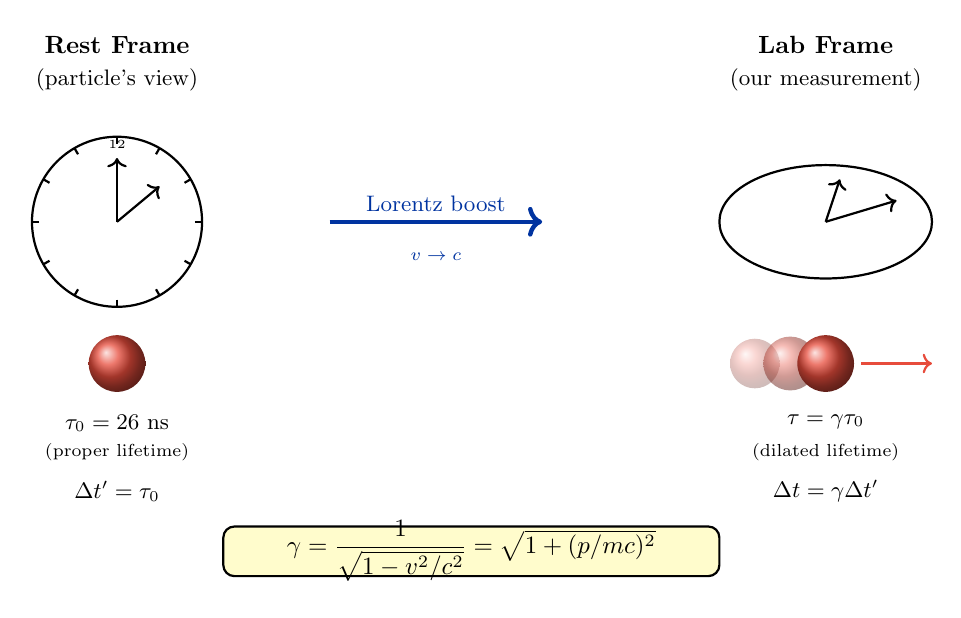
\begin{tikzpicture}[scale=0.9, transform shape]

% Left panel: Rest frame
\begin{scope}[shift={(-5, 0)}]
\node[font=\bfseries] at (0, 3.5) {Rest Frame};
\node[font=\small] at (0, 3) {(particle's view)};

% Clock
\draw[thick] (0, 1) circle (1.2cm);
\draw[thick, ->] (0, 1) -- (0, 1.9) node[above, font=\tiny] {12};
\draw[thick, ->] (0, 1) -- (0.6, 1.5);
\foreach \angle in {0, 30, 60, 90, 120, 150, 180, 210, 240, 270, 300, 330} {
    \draw[thick] ({1.1*cos(\angle)}, {1+1.1*sin(\angle)}) -- ({1.2*cos(\angle)}, {1+1.2*sin(\angle)});
}

% Particle
\shade[ball color=pionred] (0, -1) circle (0.4cm);
\node[below, font=\small] at (0, -1.6) {$\tau_0 = 26$ ns};
\node[below, font=\scriptsize] at (0, -2) {(proper lifetime)};

% Equation
\node[font=\small] at (0, -2.8) {$\Delta t' = \tau_0$};
\end{scope}

% Arrow between frames
\draw[->, ultra thick, cernblue] (-2, 1) -- (1, 1) node[midway, above, font=\small] {Lorentz boost};
\node[font=\scriptsize, cernblue] at (-0.5, 0.5) {$v \to c$};

% Right panel: Lab frame
\begin{scope}[shift={(5, 0)}]
\node[font=\bfseries] at (0, 3.5) {Lab Frame};
\node[font=\small] at (0, 3) {(our measurement)};

% Stretched clock (ellipse)
\draw[thick] (0, 1) ellipse (1.5cm and 0.8cm);
\draw[thick, ->] (0, 1) -- (0.2, 1.6);
\draw[thick, ->] (0, 1) -- (1, 1.3);

% Moving particle with motion blur
\shade[ball color=pionred, opacity=0.3] (-1, -1) circle (0.35cm);
\shade[ball color=pionred, opacity=0.5] (-0.5, -1) circle (0.38cm);
\shade[ball color=pionred] (0, -1) circle (0.4cm);
\draw[->, thick, pionred] (0.5, -1) -- (1.5, -1);

\node[below, font=\small] at (0, -1.6) {$\tau = \gamma \tau_0$};
\node[below, font=\scriptsize] at (0, -2) {(dilated lifetime)};

% Equation
\node[font=\small] at (0, -2.8) {$\Delta t = \gamma \Delta t'$};
\end{scope}

% Bottom: Key equation box
\draw[thick, rounded corners, fill=yellow!20] (-3.5, -4) rectangle (3.5, -3.3);
\node at (0, -3.65) {$\gamma = \dfrac{1}{\sqrt{1 - v^2/c^2}} = \sqrt{1 + (p/mc)^2}$};

\end{tikzpicture}
\caption{Time dilation concept: A pion with proper lifetime $\tau_0 = 26$ ns lives longer in the lab frame by factor $\gamma$. At 8 GeV/c, $\gamma_\pi = 57.3$, so observed lifetime $\tau = 1.49\ \mu$s.}
\label{fig:timedilation}
\end{figure}

\subsection{Novelty of the Comparative Null-Test Approach}

Although relativistic time dilation has been verified independently for many particle species, these tests have almost exclusively measured \textbf{one species at a time} and inferred universality by comparing extracted lifetimes to external reference values. In contrast, our experiment performs a \textbf{direct, simultaneous comparison} of pion and kaon decay-in-flight \textbf{under identical beam conditions, momentum, geometry, and detector response}, using the \textit{shape collapse of normalized survival curves} as the primary observable. This comparative \textbf{null-test} does not rely on external lifetime values or global fits and instead asks a distinct experimental question: \textit{do different particle species exhibit identical time dilation when measured side-by-side?} To our knowledge, this specific methodology, namely testing universality by direct curve comparison rather than parameter extraction, has not previously been implemented in a controlled beam experiment, making the novelty of this work methodological rather than result-driven.

\subsection{Potential Physics Beyond Standard Relativity}

If special relativity is \textit{not} exactly universal, several theoretical scenarios predict deviations:

\begin{itemize}
    \item \textbf{Mass-dependent Lorentz violation:} Some quantum gravity theories propose $\gamma_{\text{modified}} = \gamma_{\text{SR}} (1 + \alpha m^2/M_{\text{Pl}}^2)$
    \item \textbf{Composite vs.\ fundamental:} Kaons (quark composites) might differ from fundamental particles
\end{itemize}

With 4.7$\times$ mass ratio and 2--3\% precision, we can detect 1\% violations at 5$\sigma$ confidence.

% ============ DIAGRAM 5: DECAY CHANNELS ============
\begin{figure}[htbp]
\centering
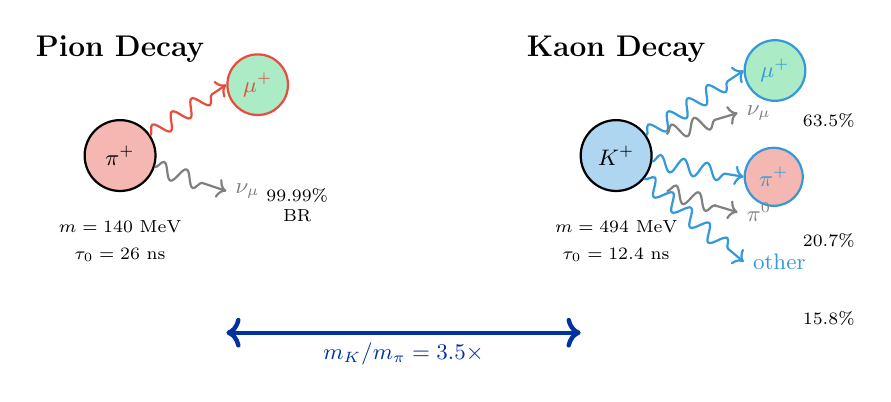
\begin{tikzpicture}[scale=0.9, transform shape,
    particle/.style={circle, draw, thick, minimum size=1cm, font=\small\bfseries},
    decay/.style={->, thick, decorate, decoration={snake, amplitude=1mm, segment length=3mm, post length=2mm}}
]

% PION DECAY
\begin{scope}[shift={(-5, 0)}]
\node[font=\bfseries\large] at (0, 2.5) {Pion Decay};
\node[particle, fill=pionred!40] (pi) at (0, 1) {$\pi^+$};
\node[font=\scriptsize] at (0, 0) {$m = 140$ MeV};
\node[font=\scriptsize] at (0, -0.4) {$\tau_0 = 26$ ns};

\draw[decay, pionred] (pi) -- ++(1.5, 1) node[right, particle, fill=muongreen!40, minimum size=0.8cm] {$\mu^+$};
\draw[decay, gray] (pi) -- ++(1.5, -0.5) node[right, font=\small] {$\nu_\mu$};

\node[font=\scriptsize, align=center] at (2.5, 0.3) {99.99\%\\BR};
\end{scope}

% KAON DECAY
\begin{scope}[shift={(2, 0)}]
\node[font=\bfseries\large] at (0, 2.5) {Kaon Decay};
\node[particle, fill=kaonblue!40] (k) at (0, 1) {$K^+$};
\node[font=\scriptsize] at (0, 0) {$m = 494$ MeV};
\node[font=\scriptsize] at (0, -0.4) {$\tau_0 = 12.4$ ns};

% Multiple decay modes
\draw[decay, kaonblue] (k) -- ++(1.8, 1.2) node[right, particle, fill=muongreen!40, minimum size=0.7cm] {$\mu^+$};
\draw[decay, gray] (k.east) ++(0.2, 0.3) -- ++(1, 0.3) node[right, font=\small] {$\nu_\mu$};
\node[font=\scriptsize] at (3, 1.5) {63.5\%};

\draw[decay, kaonblue] (k) -- ++(1.8, -0.3) node[right, particle, fill=pionred!40, minimum size=0.7cm] {$\pi^+$};
\draw[decay, gray] (k.east) ++(0.2, -0.5) -- ++(1, -0.3) node[right, font=\small] {$\pi^0$};
\node[font=\scriptsize] at (3, -0.2) {20.7\%};

\draw[decay, kaonblue] (k) -- ++(1.8, -1.5) node[right, font=\small] {other};
\node[font=\scriptsize] at (3, -1.3) {15.8\%};
\end{scope}

% Mass comparison arrow
\draw[<->, ultra thick, cernblue] (-3.5, -1.5) -- (1.5, -1.5) node[midway, below, font=\small\bfseries] {$m_K/m_\pi = 3.5\times$};

\end{tikzpicture}
\caption{Primary decay channels for pions and kaons. Both predominantly decay to muons, enabling clean detection of the decay vertex via the daughter muon trajectory.}
\label{fig:decays}
\end{figure}

\section{Impact}

\subsection{Testing Assumptions vs.\ Replicating Measurements}

This experiment differs fundamentally from previous time dilation tests:

\begin{center}
\begin{tabular}{p{5.5cm}p{5.5cm}}
\toprule
\textbf{Traditional Approach} & \textbf{Our Approach} \\
\midrule
Measure $\tau_0$ for one species & Compare two species simultaneously \\
Goal: Confirm known lifetime & Goal: Test universality assumption \\
Already done thousands of times & Never done in controlled beam \\
Educational (replicating results) & Scientific (testing hypothesis) \\
\bottomrule
\end{tabular}
\end{center}

\textbf{Key distinction:} We're not measuring what is known; instead, we are testing what's assumed.

\subsection{Novel Experimental Methodology}

Our comparative approach offers methodological advantages:
\begin{itemize}
    \item \textbf{Systematic cancellation:} Beam fluctuations affect both species equally → cancel in ratios
    \item \textbf{Self-calibration:} Muon flat reference validates detection efficiency
    \item \textbf{Null test:} Looking for agreement is more robust than extracting absolute values
\end{itemize}

This methodology can be applied to other physics tests where universality is assumed but not verified.

\section{Methodology}

\subsection{Facility and Beam Configuration}

We request CERN's PS T9 beamline configured for positive hadrons at 8 GeV/c. This provides:
\begin{itemize}
    \item \textbf{Primary beam:} Pions (10$^4$/spill, 95\%)
    \item \textbf{Kaon contamination:} 500 K$^+$/spill (5\% of beam)
    \item \textbf{Muon production:} $\sim$200 $\mu^+$/spill from $\pi \rightarrow \mu\nu$ decay
\end{itemize}

\textbf{Facility choice:} CERN PS is the only BL4S facility providing multi-GeV hadron beams. DESY provides electrons/positrons only, making this measurement impossible there.

\begin{center}
\small
\begin{tabular}{@{}llll@{}}
\toprule
\textbf{Parameter} & \textbf{Specification} & \textbf{Source} \\
\midrule
Beam momentum & 8.0 $\pm$ 0.1 GeV/c & PS T9 standard \\
Beam intensity & $10^4$ particles/spill & Adjustable \\
Spill rate & 1 Hz (typical) & 48 s cycle \\
Station 1 position & $x = 0$ m (fixed) & Reference point \\
Station 2 positions & $x = 5, 10, 15$ m & Movable \\
Flight path accuracy & $\pm$1 cm & Survey grade \\
Angular acceptance & $\pm$5 mrad & Collimation \\
\bottomrule
\end{tabular}
\end{center}

% ============ DIAGRAM 1: BEAMLINE SCHEMATIC ============
\begin{figure}[htbp]
\centering
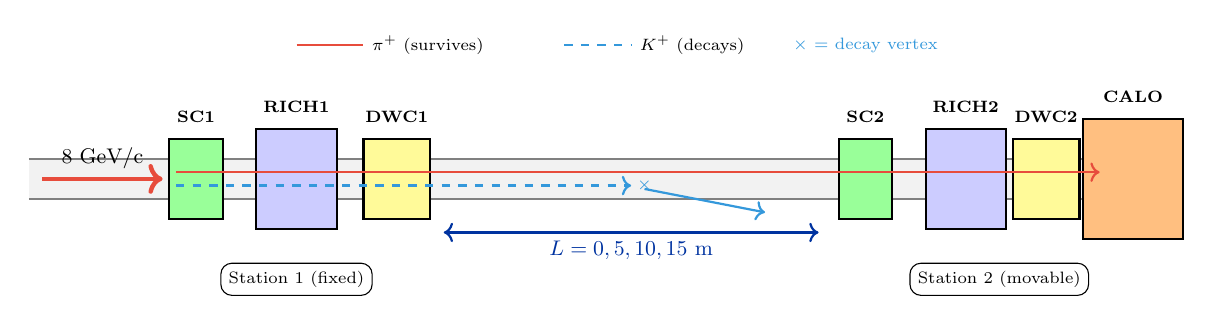
\begin{tikzpicture}[scale=0.85, transform shape,
    detector/.style={rectangle, draw=black, thick, minimum width=0.8cm, minimum height=1.2cm},
    scint/.style={detector, fill=green!40},
    rich/.style={detector, fill=blue!20, minimum width=1.2cm, minimum height=1.5cm},
    dwc/.style={detector, fill=yellow!40, minimum width=1cm},
    calo/.style={detector, fill=orange!50, minimum width=1.5cm, minimum height=1.8cm},
    particle/.style={->, thick, decorate, decoration={snake, amplitude=0.3mm, segment length=2mm}},
    beam/.style={->, ultra thick, pionred}
]

% Beam pipe
\fill[gray!10] (-1, -0.3) rectangle (16, 0.3);
\draw[gray, thick] (-1, -0.3) -- (16, -0.3);
\draw[gray, thick] (-1, 0.3) -- (16, 0.3);

% Beam arrow
\draw[beam] (-0.8, 0) -- (1, 0) node[above, midway, black] {\small 8 GeV/c};

% Station 1 (z = 0.5m)
\node[scint] (sc1) at (1.5, 0) {};
\node[above=0.1cm of sc1, font=\scriptsize\bfseries] {SC1};

\node[rich] (rich1) at (3, 0) {};
\node[above=0.1cm of rich1, font=\scriptsize\bfseries] {RICH1};

\node[dwc] (dwc1) at (4.5, 0) {};
\node[above=0.1cm of dwc1, font=\scriptsize\bfseries] {DWC1};

% Flight path (variable)
\draw[<->, thick, cernblue] (5.2, -0.8) -- (10.8, -0.8) node[midway, below, font=\small] {$L = 0, 5, 10, 15$ m};

% Station 2 (movable)
\node[scint] (sc2) at (11.5, 0) {};
\node[above=0.1cm of sc2, font=\scriptsize\bfseries] {SC2};

\node[rich] (rich2) at (13, 0) {};
\node[above=0.1cm of rich2, font=\scriptsize\bfseries] {RICH2};

\node[dwc] (dwc2) at (14.2, 0) {};
\node[above=0.1cm of dwc2, font=\scriptsize\bfseries] {DWC2};

\node[calo] (cal) at (15.5, 0) {};
\node[above=0.1cm of cal, font=\scriptsize\bfseries] {CALO};

% Particle trajectories
\draw[pionred, thick, ->] (1.2, 0.1) -- (15, 0.1);
\draw[kaonblue, thick, ->, dashed] (1.2, -0.1) -- (8, -0.1);
\node[kaonblue] at (8.2, -0.1) {\scriptsize $\times$};
\draw[kaonblue, thick, ->] (8.2, -0.15) -- (10, -0.5);

% Labels
\node[draw, rounded corners, fill=white, font=\scriptsize] at (3, -1.5) {Station 1 (fixed)};
\node[draw, rounded corners, fill=white, font=\scriptsize] at (13.5, -1.5) {Station 2 (movable)};

% Legend
\begin{scope}[shift={(0, 2)}]
\draw[pionred, thick] (3, 0) -- (4, 0) node[right, black, font=\scriptsize] {$\pi^+$ (survives)};
\draw[kaonblue, thick, dashed] (7, 0) -- (8, 0) node[right, black, font=\scriptsize] {$K^+$ (decays)};
\node[kaonblue, font=\scriptsize] at (11.5, 0) {$\times$ = decay vertex};
\end{scope}

\end{tikzpicture}
\caption{Schematic of the T9 beamline experimental setup. Station 1 remains fixed while Station 2 moves to distances $L = 0, 5, 10, 15$ m to measure survival fraction vs.\ flight path.}
\label{fig:beamline}
\end{figure}

At fixed momentum $p = 8$ GeV/c, each particle has different velocity:
\begin{align}
\beta_\pi &= 0.99985 \quad (\gamma = 57.3) \\
\beta_K &= 0.99810 \quad (\gamma = 16.2) \\
\beta_\mu &= 0.99991 \quad (\gamma = 75.7)
\end{align}

% ============ DIAGRAM 6: CHERENKOV PRINCIPLE ============
\begin{figure}[htbp]
\centering
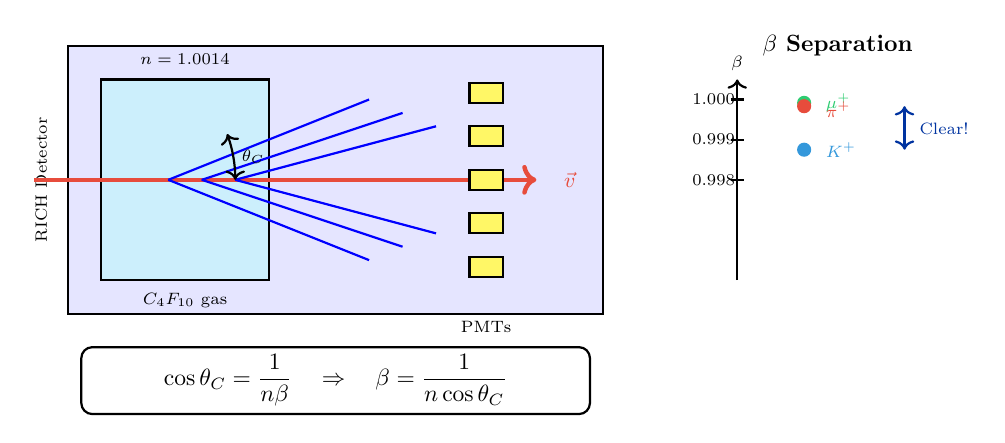
\begin{tikzpicture}[scale=0.85, transform shape]

% RICH detector box
\fill[blue!10] (0, -2) rectangle (8, 2);
\draw[thick] (0, -2) rectangle (8, 2);
\node[font=\scriptsize, rotate=90] at (-0.4, 0) {RICH Detector};

% Radiator medium
\fill[cyan!20] (0.5, -1.5) rectangle (3, 1.5);
\draw[thick] (0.5, -1.5) rectangle (3, 1.5);
\node[font=\scriptsize] at (1.75, -1.8) {$C_4F_{10}$ gas};
\node[font=\scriptsize] at (1.75, 1.8) {$n = 1.0014$};

% Particle trajectory
\draw[pionred, ultra thick, ->] (-0.5, 0) -- (7, 0);
\node[pionred, font=\small] at (7.5, 0) {$\vec{v}$};

% Cherenkov cone
\draw[blue, thick] (1.5, 0) -- (4.5, 1.2);
\draw[blue, thick] (1.5, 0) -- (4.5, -1.2);
\draw[blue, thick] (2, 0) -- (5, 1);
\draw[blue, thick] (2, 0) -- (5, -1);
\draw[blue, thick] (2.5, 0) -- (5.5, 0.8);
\draw[blue, thick] (2.5, 0) -- (5.5, -0.8);

% Photon detectors (PMTs)
\foreach \y in {-1.3, -0.65, 0, 0.65, 1.3} {
    \fill[yellow!60] (6, \y-0.15) rectangle (6.5, \y+0.15);
    \draw[thick] (6, \y-0.15) rectangle (6.5, \y+0.15);
}
\node[font=\scriptsize] at (6.25, -2.2) {PMTs};

% Cherenkov angle annotation
\draw[<->, thick] (2.5, 0) arc (0:20:2) node[midway, right, font=\scriptsize] {$\theta_C$};

% Formula box
\draw[thick, rounded corners, fill=white] (0.2, -3.5) rectangle (7.8, -2.5);
\node at (4, -3) {$\cos\theta_C = \dfrac{1}{n\beta} \quad \Rightarrow \quad \beta = \dfrac{1}{n\cos\theta_C}$};

% Separation illustration (right side)
\begin{scope}[shift={(10, 0)}]
\node[font=\bfseries] at (1.5, 2) {$\beta$ Separation};

% Beta scale
\draw[thick, ->] (0, -1.5) -- (0, 1.5) node[above, font=\scriptsize] {$\beta$};
\draw[thick] (-0.1, 1.2) -- (0.1, 1.2) node[left, font=\scriptsize] {1.000};
\draw[thick] (-0.1, 0.6) -- (0.1, 0.6) node[left, font=\scriptsize] {0.999};
\draw[thick] (-0.1, 0) -- (0.1, 0) node[left, font=\scriptsize] {0.998};

% Particle markers with error bars
\fill[muongreen] (1, 1.15) circle (3pt); \node[right, muongreen, font=\scriptsize] at (1.2, 1.15) {$\mu^+$};
\fill[pionred] (1, 1.1) circle (3pt); \node[right, pionred, font=\scriptsize] at (1.2, 1.05) {$\pi^+$};
\fill[kaonblue] (1, 0.45) circle (3pt); \node[right, kaonblue, font=\scriptsize] at (1.2, 0.45) {$K^+$};

% Separation arrow
\draw[<->, thick, cernblue] (2.5, 0.45) -- (2.5, 1.1);
\node[font=\scriptsize, cernblue, right] at (2.6, 0.77) {Clear!};
\end{scope}

\end{tikzpicture}
\caption{RICH detector principle: Cherenkov photons emitted at angle $\theta_C = \arccos(1/n\beta)$ allow velocity measurement. At 8 GeV/c, kaons ($\beta_K = 0.998$) are clearly separated from pions/muons ($\beta > 0.9998$).}
\label{fig:cherenkov}
\end{figure}

\textbf{Particle identification algorithm (two-stage):}

\begin{center}
\small
\begin{tabular}{p{6cm}|p{6cm}}
\toprule
\textbf{Stage 1: RICH Velocity Measurement} & \textbf{Stage 2: Energy + Topology} \\
\midrule
\textbullet\ Measure Cherenkov angle: $\cos\theta_C = 1/(n\beta)$ & \textbullet\ Calorimeter measures total energy \\
\textbullet\ Extract $\beta$ with precision $\Delta\beta/\beta \sim 10^{-3}$ & \textbullet\ Pions: stable over 15 m, primary vertex \\
\textbullet\ Kaons clearly separated: $\beta_K < 0.999$ & \textbullet\ Muons: secondary vertices visible \\
\textbullet\ Pions/muons degenerate: $\beta_{\pi,\mu} > 0.9998$ & \textbullet\ DWC tracking identifies decay-in-flight kinks \\
\bottomrule
\end{tabular}
\end{center}

\begin{center}
\small
\begin{tabular}{@{}lcc@{}}
\toprule
\textbf{Expected Performance} & \textbf{Efficiency} & \textbf{Notes} \\
\midrule
Kaon ID & $>$95\% & Clean RICH separation \\
Pion ID & $>$90\% & Topology + timing \\
Cross-contamination & $<$2\% & Combined cuts \\
\bottomrule
\end{tabular}
\end{center}

% ============ DIAGRAM 3: PARTICLE ID FLOWCHART ============
\begin{figure}[htbp]
\centering
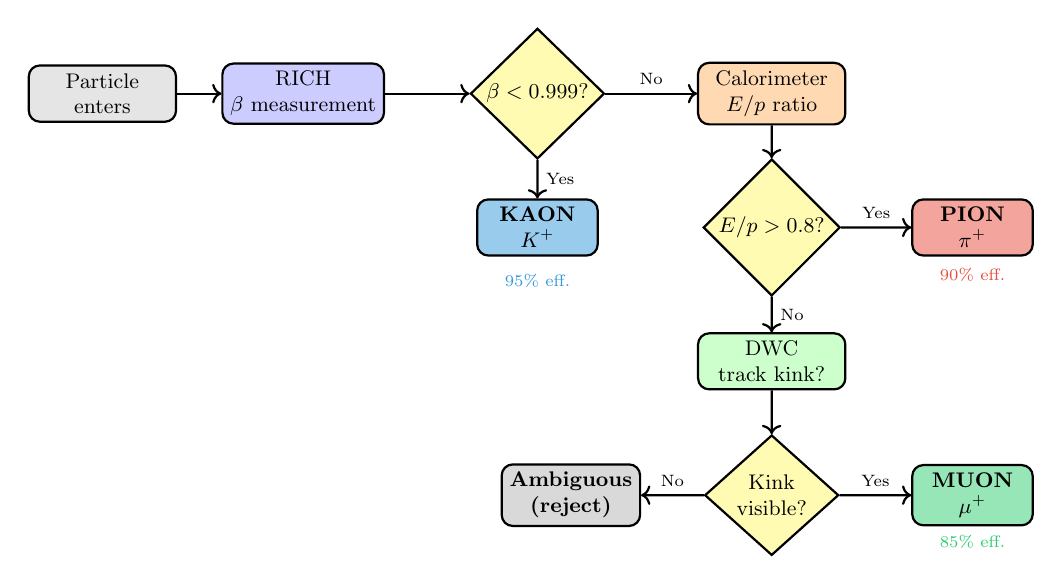
\begin{tikzpicture}[scale=0.85, transform shape,
    block/.style={rectangle, draw, thick, rounded corners, minimum width=2.2cm, minimum height=0.8cm, align=center, font=\small},
    decision/.style={diamond, draw, thick, minimum width=2cm, minimum height=1cm, align=center, font=\small, inner sep=1pt},
    result/.style={rectangle, draw, thick, rounded corners, minimum width=1.8cm, minimum height=0.7cm, align=center, font=\small\bfseries},
    arrow/.style={->, thick}
]

% Start
\node[block, fill=gray!20] (start) at (0, 0) {Particle\\enters};

% RICH measurement
\node[block, fill=blue!20] (rich) at (3, 0) {RICH\\$\beta$ measurement};
\draw[arrow] (start) -- (rich);

% First decision: beta < 0.999?
\node[decision, fill=yellow!30] (dec1) at (6.5, 0) {$\beta < 0.999$?};
\draw[arrow] (rich) -- (dec1);

% Kaon branch
\node[result, fill=kaonblue!50] (kaon) at (6.5, -2) {KAON\\$K^+$};
\draw[arrow] (dec1) -- node[right, font=\scriptsize] {Yes} (kaon);

% Continue to Stage 2
\node[block, fill=orange!30] (calo) at (10, 0) {Calorimeter\\$E/p$ ratio};
\draw[arrow] (dec1) -- node[above, font=\scriptsize] {No} (calo);

% Second decision: E/p
\node[decision, fill=yellow!30] (dec2) at (10, -2) {$E/p > 0.8$?};
\draw[arrow] (calo) -- (dec2);

% Pion branch
\node[result, fill=pionred!50] (pion) at (13, -2) {PION\\$\pi^+$};
\draw[arrow] (dec2) -- node[above, font=\scriptsize] {Yes} (pion);

% DWC check
\node[block, fill=green!20] (dwc) at (10, -4) {DWC\\track kink?};
\draw[arrow] (dec2) -- node[right, font=\scriptsize] {No} (dwc);

% Third decision
\node[decision, fill=yellow!30] (dec3) at (10, -6) {Kink\\visible?};
\draw[arrow] (dwc) -- (dec3);

% Muon branch
\node[result, fill=muongreen!50] (muon) at (13, -6) {MUON\\$\mu^+$};
\draw[arrow] (dec3) -- node[above, font=\scriptsize] {Yes} (muon);

% Ambiguous
\node[result, fill=gray!30] (ambig) at (7, -6) {Ambiguous\\(reject)};
\draw[arrow] (dec3) -- node[above, font=\scriptsize] {No} (ambig);

% Efficiency labels
\node[font=\scriptsize, kaonblue] at (6.5, -2.8) {95\% eff.};
\node[font=\scriptsize, pionred] at (13, -2.7) {90\% eff.};
\node[font=\scriptsize, muongreen] at (13, -6.7) {85\% eff.};

\end{tikzpicture}
\caption{Two-stage particle identification algorithm. RICH clearly separates kaons ($\beta < 0.999$). Pions and muons require additional calorimeter and tracking information.}
\label{fig:pidflow}
\end{figure}

\subsection{Note on Muons as Calibration Reference}

\textbf{Critical clarification:} While muons are present in the beam from pion decay, their enormous decay length ($\lambda_\mu \approx 49,900$ m at 8 GeV/c) means \textbf{essentially zero decay} over our 15 m flight path (survival = 99.97\%). 

We will use muons as a \textbf{non-decaying reference species} to validate detection efficiency and particle ID, not as a third decay measurement. A constant muon rate $N_\mu(x)/N_\mu(0) \approx 1.000$ across all distances confirms our systematics are under control.

\textbf{Our primary universality test compares pions and kaons}, which span a 4.7$\times$ mass ratio, which is sufficient to test for mass-dependent Lorentz violations with high sensitivity.

\subsection{Measurement Protocol}

\begin{center}
\small
\begin{tabular}{@{}clp{8cm}@{}}
\toprule
\textbf{Days} & \textbf{Phase} & \textbf{Activities} \\
\midrule
1--2 & Installation \& Calibration & Mount detectors at T9 positions; configure RICH for optimal $\beta$ resolution; calibrate calorimeter energy response; verify trigger logic ($T =$ SC1 $\land$ SC2, 5 ns window) \\
\midrule
3--5 & Particle ID Validation & Fixed beam (8 GeV/c), Station 2 at 0 m; collect 50,000 pions, 2,500 kaons, 1,000 muons; plot $\beta$ vs.\ $E_{\text{cal}}$; determine ID efficiency and cross-contamination; validate muon topology \\
\midrule
6--9 & Decay Measurements & Move Station 2 to $x = 5, 10, 15$ m; collect 1000 spills per position ($\sim$8 hours each); record particle ID, flight distance, time-of-flight; bin data by species; monitor muon rate \\
\midrule
10 & Analysis \& Test & Extract survival curves; normalize by decay length $\lambda_i = \beta_i c \gamma_i \tau_{0,i}$; test if $\pi$ and $K$ curves collapse; $\chi^2$ goodness-of-fit; verify muon calibration \\
\bottomrule
\end{tabular}
\end{center}

% ============ DIAGRAM 9: EXPERIMENT TIMELINE ============
\begin{figure}[htbp]
\centering
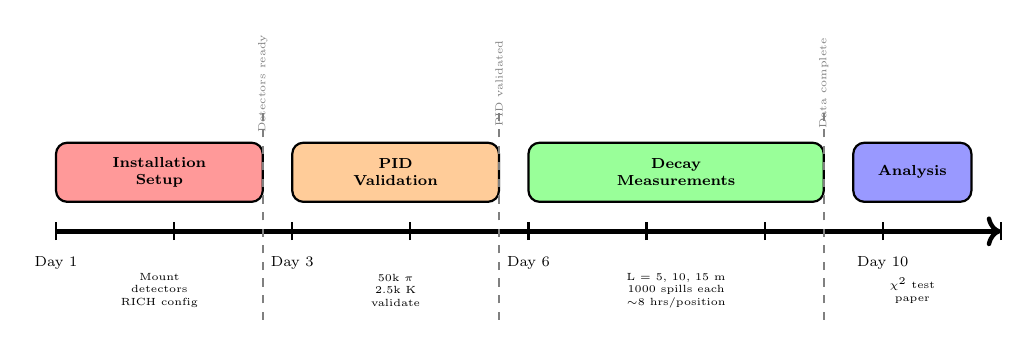
\begin{tikzpicture}[scale=0.75, transform shape]

% Timeline axis
\draw[ultra thick, ->] (0, 0) -- (16, 0);
\foreach \x in {0, 2, 4, 6, 8, 10, 12, 14, 16} {
    \draw[thick] (\x, -0.15) -- (\x, 0.15);
}
\node[below] at (0, -0.3) {\scriptsize Day 1};
\node[below] at (4, -0.3) {\scriptsize Day 3};
\node[below] at (8, -0.3) {\scriptsize Day 6};
\node[below] at (14, -0.3) {\scriptsize Day 10};

% Phase blocks
% Phase 1: Installation (Days 1-2)
\fill[red!40, rounded corners] (0, 0.5) rectangle (3.5, 1.5);
\draw[thick, rounded corners] (0, 0.5) rectangle (3.5, 1.5);
\node[font=\scriptsize\bfseries, align=center] at (1.75, 1) {Installation\\Setup};

% Phase 2: Calibration (Days 3-5)
\fill[orange!40, rounded corners] (4, 0.5) rectangle (7.5, 1.5);
\draw[thick, rounded corners] (4, 0.5) rectangle (7.5, 1.5);
\node[font=\scriptsize\bfseries, align=center] at (5.75, 1) {PID\\Validation};

% Phase 3: Data taking (Days 6-9)
\fill[green!40, rounded corners] (8, 0.5) rectangle (13, 1.5);
\draw[thick, rounded corners] (8, 0.5) rectangle (13, 1.5);
\node[font=\scriptsize\bfseries, align=center] at (10.5, 1) {Decay\\Measurements};

% Phase 4: Analysis (Day 10)
\fill[blue!40, rounded corners] (13.5, 0.5) rectangle (15.5, 1.5);
\draw[thick, rounded corners] (13.5, 0.5) rectangle (15.5, 1.5);
\node[font=\scriptsize\bfseries, align=center] at (14.5, 1) {Analysis};

% Details below
\node[font=\tiny, align=center] at (1.75, -1) {Mount\\detectors\\RICH config};
\node[font=\tiny, align=center] at (5.75, -1) {50k $\pi$\\2.5k K\\validate};
\node[font=\tiny, align=center] at (10.5, -1) {L = 5, 10, 15 m\\1000 spills each\\$\sim$8 hrs/position};
\node[font=\tiny, align=center] at (14.5, -1) {$\chi^2$ test\\paper};

% Milestones
\draw[thick, dashed, gray] (3.5, -1.5) -- (3.5, 2);
\node[font=\tiny, gray, rotate=90] at (3.5, 2.5) {Detectors ready};
\draw[thick, dashed, gray] (7.5, -1.5) -- (7.5, 2);
\node[font=\tiny, gray, rotate=90] at (7.5, 2.5) {PID validated};
\draw[thick, dashed, gray] (13, -1.5) -- (13, 2);
\node[font=\tiny, gray, rotate=90] at (13, 2.5) {Data complete};

\end{tikzpicture}
\caption{Ten-day experiment timeline showing the four main phases: detector installation, particle ID validation, decay measurements at three flight distances, and preliminary analysis.}
\label{fig:timeline}
\end{figure}

\section{Expected Outcomes}

\subsection{Theoretical Predictions}

At 8 GeV/c, the decay lengths differ dramatically:
\begin{itemize}
    \item \textbf{Pions:} $\lambda_\pi = 447$ m (1.2\% decay at 5 m, 3.3\% at 15 m)
    \item \textbf{Kaons:} $\lambda_K = 60$ m (8.0\% decay at 5 m, 22.1\% at 15 m)
    \item \textbf{Muons:} $\lambda_\mu = 49,900$ m (0.03\% decay at 15 m, which is negligible)
\end{itemize}

% ============ DIAGRAM 4: SURVIVAL CURVES ============
\begin{figure}[htbp]
\centering
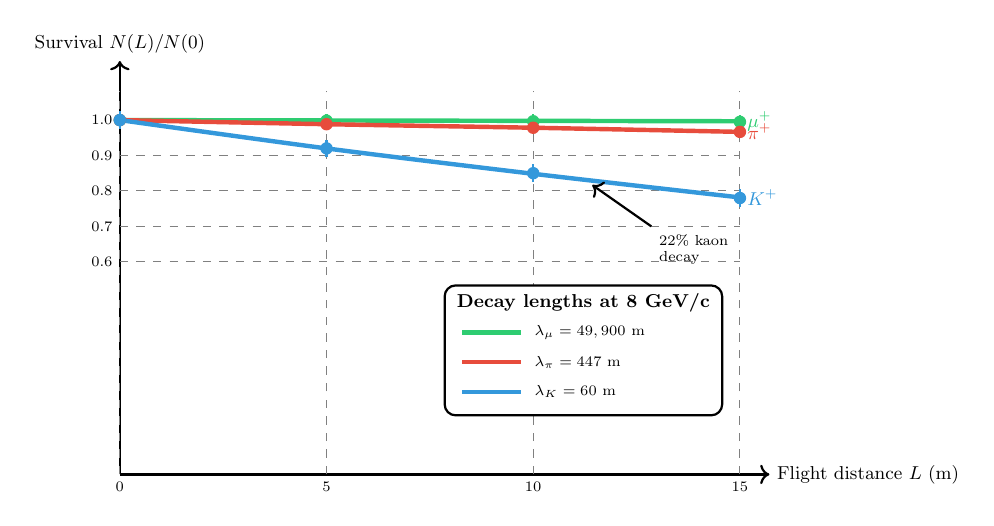
\begin{tikzpicture}[scale=0.75, transform shape]

% Axes
\draw[thick, ->] (0, 0) -- (11, 0) node[right, font=\small] {Flight distance $L$ (m)};
\draw[thick, ->] (0, 0) -- (0, 7) node[above, font=\small] {Survival $N(L)/N(0)$};

% Grid
\foreach \x in {0, 5, 10, 15} {
    \draw[gray, thin, dashed] (\x*0.7, 0) -- (\x*0.7, 6.5);
    \node[below, font=\scriptsize] at (\x*0.7, 0) {\x};
}
\foreach \y in {0.6, 0.7, 0.8, 0.9, 1.0} {
    \draw[gray, thin, dashed] (0, \y*6) -- (10.5, \y*6);
    \node[left, font=\scriptsize] at (0, \y*6) {\y};
}

% Muon curve (nearly flat)
\draw[muongreen, ultra thick] (0, 6) -- (10.5, 5.98);
\node[muongreen, font=\small\bfseries, right] at (10.5, 5.98) {$\mu^+$};

% Pion curve (slow decay)
\draw[pionred, ultra thick] plot[smooth] coordinates {
    (0, 6) (3.5, 5.93) (7, 5.87) (10.5, 5.80)
};
\node[pionred, font=\small\bfseries, right] at (10.5, 5.80) {$\pi^+$};

% Kaon curve (faster decay)
\draw[kaonblue, ultra thick] plot[smooth] coordinates {
    (0, 6) (3.5, 5.52) (7, 5.09) (10.5, 4.69)
};
\node[kaonblue, font=\small\bfseries, right] at (10.5, 4.69) {$K^+$};

% Data points with error bars
\foreach \x/\ymu/\ypi/\yk in {0/6/6/6, 3.5/5.99/5.93/5.52, 7/5.98/5.87/5.10, 10.5/5.97/5.80/4.68} {
    % Muon
    \fill[muongreen] (\x, \ymu) circle (3pt);
    \draw[muongreen, thick] (\x, \ymu-0.12) -- (\x, \ymu+0.12);
    % Pion
    \fill[pionred] (\x, \ypi) circle (3pt);
    \draw[pionred, thick] (\x, \ypi-0.08) -- (\x, \ypi+0.08);
    % Kaon
    \fill[kaonblue] (\x, \yk) circle (3pt);
    \draw[kaonblue, thick] (\x, \yk-0.15) -- (\x, \yk+0.15);
}

% Legend box
\draw[thick, rounded corners, fill=white] (5.5, 1) rectangle (10.2, 3.2);
\node[font=\small\bfseries] at (7.85, 2.9) {Decay lengths at 8 GeV/c};
\draw[muongreen, ultra thick] (5.8, 2.4) -- (6.8, 2.4); \node[right, font=\scriptsize] at (6.9, 2.4) {$\lambda_\mu = 49,900$ m};
\draw[pionred, ultra thick] (5.8, 1.9) -- (6.8, 1.9); \node[right, font=\scriptsize] at (6.9, 1.9) {$\lambda_\pi = 447$ m};
\draw[kaonblue, ultra thick] (5.8, 1.4) -- (6.8, 1.4); \node[right, font=\scriptsize] at (6.9, 1.4) {$\lambda_K = 60$ m};

% Annotation
\draw[<-, thick] (8, 4.9) -- (9, 4.2) node[below right, font=\scriptsize, align=left] {22\% kaon\\decay};

\end{tikzpicture}
\caption{Expected survival curves for pions, kaons, and muons at 8 GeV/c. Kaons show significant decay (22\% at 15 m) due to shorter decay length. Muons remain nearly constant (calibration reference).}
\label{fig:survival}
\end{figure}

\subsection{Statistical Precision}

Expected event counts (1000 spills per distance, 3 distances):
\begin{itemize}
    \item \textbf{Pions:} $\sim$10$^7$ total events → statistical precision $\pm$0.01\%
    \item \textbf{Kaons:} $\sim$5$\times$10$^5$ events → statistical precision $\pm$0.14\%
    \item \textbf{Muons:} $\sim$2$\times$10$^5$ events → flat reference (calibration)
\end{itemize}

\subsection{Systematic Uncertainties}

\begin{center}
\small
\begin{tabular}{@{}lll@{}}
\toprule
\textbf{Source} & \textbf{Contribution} & \textbf{Mitigation} \\
\midrule
Distance calibration & $\pm$1.0\% & Survey-grade measurement \\
Beam energy spread & $\pm$0.8\% & PS momentum bite specification \\
PID efficiency & $\pm$1.5\% & Large validation sample (50k events) \\
Trigger acceptance & $\pm$1.2\% & Cross-trigger studies with muons \\
Background subtraction & $\pm$0.5\% & Empty-target runs \\
Time-of-flight resolution & $\pm$0.3\% & Clock calibration \\
\midrule
\textbf{Total systematic (quadrature)} & \textbf{$\pm$2.4\%} & Conservative estimate \\
Statistical (per point) & $\pm$1.0\% & Sufficient beam time \\
\midrule
\textbf{Combined uncertainty} & \textbf{$\pm$2.6\%} & Enables 5$\sigma$ test \\
\bottomrule
\end{tabular}
\end{center}

% ============ DIAGRAM 7: ERROR BUDGET PIE CHART ============
\begin{figure}[htbp]
\centering
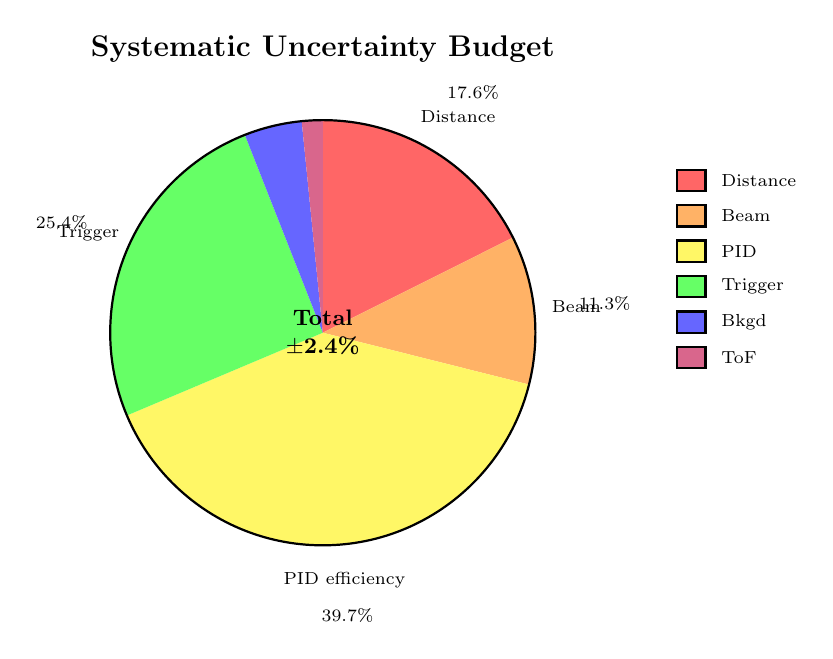
\begin{tikzpicture}[scale=0.9, transform shape]

% Title
\node[font=\bfseries\large] at (0, 4) {Systematic Uncertainty Budget};

% Pie chart data (angles proportional to variance = error^2)
% Total variance = 1^2 + 0.8^2 + 1.5^2 + 1.2^2 + 0.5^2 + 0.3^2 = 5.67
% Percentages: 17.6%, 11.3%, 39.7%, 25.4%, 4.4%, 1.6%

\def\radius{3}

% Slice 1: Distance (17.6% = 63.4°)
\fill[red!60] (0,0) -- (90:\radius) arc (90:26.6:\radius) -- cycle;
\node at (58:\radius+0.6) {\scriptsize Distance};
\node at (58:\radius+1) {\scriptsize 17.6\%};

% Slice 2: Beam energy (11.3% = 40.7°)  
\fill[orange!60] (0,0) -- (26.6:\radius) arc (26.6:-14.1:\radius) -- cycle;
\node at (6:\radius+0.6) {\scriptsize Beam};
\node at (6:\radius+1) {\scriptsize 11.3\%};

% Slice 3: PID (39.7% = 143°)
\fill[yellow!60] (0,0) -- (-14.1:\radius) arc (-14.1:-157.1:\radius) -- cycle;
\node at (-85:\radius+0.5) {\scriptsize PID efficiency};
\node at (-85:\radius+1) {\scriptsize 39.7\%};

% Slice 4: Trigger (25.4% = 91.4°)
\fill[green!60] (0,0) -- (-157.1:\radius) arc (-157.1:-248.5:\radius) -- cycle;
\node at (-203:\radius+0.6) {\scriptsize Trigger};
\node at (-203:\radius+1) {\scriptsize 25.4\%};

% Slice 5: Background (4.4% = 15.8°)
\fill[blue!60] (0,0) -- (-248.5:\radius) arc (-248.5:-264.3:\radius) -- cycle;

% Slice 6: ToF (1.6% = 5.7°)
\fill[purple!60] (0,0) -- (-264.3:\radius) arc (-264.3:-270:\radius) -- cycle;

% Draw outline
\draw[thick] (0,0) circle (\radius);

% Center label
\node[align=center, font=\small\bfseries] at (0, 0) {Total\\$\pm$2.4\%};

% Legend
\begin{scope}[shift={(5, 2)}]
\foreach \i/\col/\txt in {0/red!60/Distance, 1/orange!60/Beam, 2/yellow!60/PID, 3/green!60/Trigger, 4/blue!60/Bkgd, 5/purple!60/ToF} {
    \fill[\col] (0, -\i*0.5) rectangle (0.4, -\i*0.5+0.3);
    \draw[thick] (0, -\i*0.5) rectangle (0.4, -\i*0.5+0.3);
    \node[right, font=\scriptsize] at (0.5, -\i*0.5+0.15) {\txt};
}
\end{scope}

\end{tikzpicture}
\caption{Breakdown of systematic uncertainties by source. PID efficiency dominates; this is mitigated by large calibration samples and redundant detectors.}
\label{fig:errors}
\end{figure}

\textbf{Sensitivity to violations:} With 2--3\% precision, we can detect:
\begin{itemize}
    \item 1\% difference in $\gamma$ between species: \textbf{5$\sigma$ detection}
    \item Mass-dependent corrections at the $10^{-2}$ level
    \item Deviations from exponential decay (non-SR effects)
\end{itemize}

This precision \textbf{exceeds previous single-particle measurements} for comparative tests and sets a new benchmark for universality verification.

\subsection{Expected Outcomes and Interpretation}

\textbf{Outcome 1: Perfect agreement (most likely)}\\
Normalized pion and kaon curves collapse within 2$\sigma$ errors. $\chi^2/$d.o.f.\ $\approx 1.0$. Muon rate remains constant.

\textbf{Conclusion:} Special relativity is universal across particle species to 2--3\% precision, confirming Einstein's prediction at a new level of rigor through direct comparison.

\textbf{Scientific value:} First direct verification of universality assumption between hadrons at fixed momentum. Publishable in \textit{American Journal of Physics} or \textit{Physics Education} as pedagogical confirmation with novel comparative methodology.

\textbf{Outcome 2: Systematic deviation}\\
Pion and kaon curves show consistent offset beyond statistical errors.

\textbf{Conclusion:} Either (a) unrecognized systematic error requiring investigation, or (b) genuinely new physics indicating mass-dependent Lorentz violation.

\textbf{Scientific value:} Would trigger theoretical analysis and follow-up experiments. Even if ultimately traced to systematics, the measurement technique is validated for future precision tests.

% ============ DIAGRAM 8: UNIVERSALITY TEST ============
\begin{figure}[htbp]
\centering
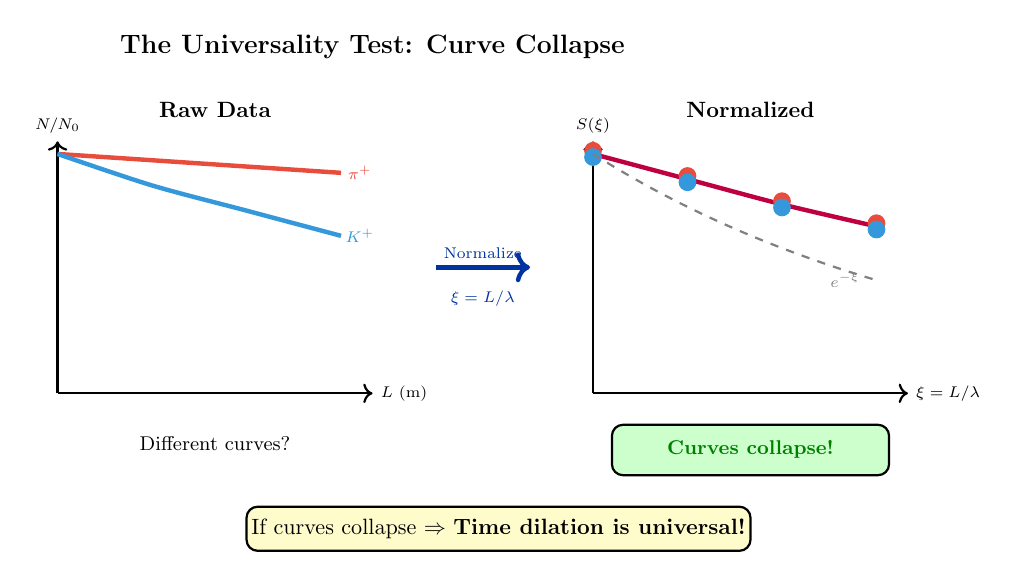
\begin{tikzpicture}[scale=0.8, transform shape]

% Title
\node[font=\bfseries\large] at (5, 5.5) {The Universality Test: Curve Collapse};

% Left panel: Raw survival curves
\begin{scope}[shift={(0, 0)}]
\node[font=\bfseries] at (2.5, 4.5) {Raw Data};

% Axes
\draw[thick, ->] (0, 0) -- (5, 0) node[right, font=\scriptsize] {$L$ (m)};
\draw[thick, ->] (0, 0) -- (0, 4) node[above, font=\scriptsize] {$N/N_0$};

% Pion curve (slow decay)
\draw[pionred, ultra thick] plot[smooth] coordinates {(0, 3.8) (1.5, 3.7) (3, 3.6) (4.5, 3.5)};
\node[pionred, font=\scriptsize] at (4.8, 3.5) {$\pi^+$};

% Kaon curve (fast decay)
\draw[kaonblue, ultra thick] plot[smooth] coordinates {(0, 3.8) (1.5, 3.3) (3, 2.9) (4.5, 2.5)};
\node[kaonblue, font=\scriptsize] at (4.8, 2.5) {$K^+$};

% Question
\node[font=\small] at (2.5, -0.8) {Different curves?};
\end{scope}

% Arrow
\draw[->, ultra thick, cernblue] (6, 2) -- (7.5, 2) node[midway, above, font=\scriptsize] {Normalize};
\node[font=\scriptsize, cernblue] at (6.75, 1.5) {$\xi = L/\lambda$};

% Right panel: Normalized curves
\begin{scope}[shift={(8.5, 0)}]
\node[font=\bfseries] at (2.5, 4.5) {Normalized};

% Axes
\draw[thick, ->] (0, 0) -- (5, 0) node[right, font=\scriptsize] {$\xi = L/\lambda$};
\draw[thick, ->] (0, 0) -- (0, 4) node[above, font=\scriptsize] {$S(\xi)$};

% Both curves collapse!
\draw[purple, ultra thick] plot[smooth] coordinates {(0, 3.8) (1.5, 3.4) (3, 3.0) (4.5, 2.65)};

% Data points overlapping
\foreach \x/\y in {0/3.8, 1.5/3.4, 3/3.0, 4.5/2.65} {
    \fill[pionred] (\x, \y+0.05) circle (4pt);
    \fill[kaonblue] (\x, \y-0.05) circle (4pt);
}

% Theory line
\draw[gray, thick, dashed] plot[domain=0:4.5, samples=30] (\x, {3.8*exp(-\x/6)});
\node[gray, font=\scriptsize] at (4, 1.8) {$e^{-\xi}$};

% Result box
\draw[thick, rounded corners, fill=green!20] (0.3, -1.3) rectangle (4.7, -0.5);
\node[font=\small\bfseries, green!50!black] at (2.5, -0.9) {Curves collapse!};
\end{scope}

% Bottom conclusion
\draw[thick, rounded corners, fill=yellow!20] (3, -2.5) rectangle (11, -1.8);
\node at (7, -2.15) {If curves collapse $\Rightarrow$ \textbf{Time dilation is universal!}};

\end{tikzpicture}
\caption{The universality test: When survival curves are normalized by decay length $\lambda = \beta c \gamma \tau_0$, pion and kaon data should collapse to the same universal exponential $S(\xi) = e^{-\xi}$ if special relativity is universal.}
\label{fig:universality}
\end{figure}


\section{Risk Assessment and Contingency}

\subsection{Technical Challenges}

\textbf{Challenge 1: Particle ID efficiency}
\begin{itemize}
    \item \textbf{Risk:} Overlapping $\beta$ distributions cause misidentification
    \item \textbf{Mitigation:} RICH + calorimeter provides redundancy; topology cuts for muons
    \item \textbf{Fallback:} If separation poor, analyze $\pi$ vs.\ $K$ only (sufficient for test)
\end{itemize}

\textbf{Challenge 2: Low kaon statistics}
\begin{itemize}
    \item \textbf{Risk:} Only 500 K$^+$/spill gives 0.14\% precision (still acceptable)
    \item \textbf{Mitigation:} Request higher beam intensity if facility permits
    \item \textbf{Acceptance:} Even 0.2\% per point sufficient for 2--3\% total precision
\end{itemize}

\textbf{Challenge 3: Systematic uncertainties accumulate}
\begin{itemize}
    \item \textbf{Risk:} Distance calibration, beam energy, PID efficiency total to 2.4\%
    \item \textbf{Mitigation:} Conservative error budget, muon calibration validates systematics
    \item \textbf{Acceptance:} 2--3\% precision still enables 5$\sigma$ test of 1\% violations
\end{itemize}

\subsection{Honest Limitations}

\textbf{This will NOT revolutionize physics.} Special relativity will almost certainly pass this test. Our contribution is:
\begin{enumerate}
    \item First direct comparative pion-kaon universality test
    \item Demonstrating comparative null-test methodology
    \item Educational value of testing fundamental assumptions
    \item Setting precision benchmark for future tests
\end{enumerate}

The value is \textbf{pedagogical and methodological}, confirming what we expect while establishing techniques for more sensitive tests.

\section{What We Hope to Take Away}

Through this experiment, we hope to gain a first-hand understanding of how fundamental physics is tested in practice, beyond textbook derivations and simulations. We want to experience how real experimental constraints, including detector limitations, background rejection, calibration, and systematic uncertainties, shape what can actually be measured, and how careful experimental design allows meaningful questions to be answered even with imperfect tools. Working with professional detectors and a live beamline would teach us how ideas are translated into hardware, triggers, data, and statistical conclusions.

Our goal is to bring the work carried out during the beam time to the standard required for submission to peer-reviewed journals such as \textit{Physics Education} or \textit{Journal of Instrumentation}, as has been achieved by previous Beamline for Schools teams.

For us personally, we would be the first generation in our families to travel internationally, work alongside PhD physicists, and handle equipment worth more than our school's entire science budgets, haha! We would have adults treat our ideas seriously rather than telling us to focus on exams first.

We hope you see eight teenagers who prepared seriously and deserve one chance to find out if their predictions match reality. We are ready.

\section{Outreach}

\subsection{Post-CERN Plans}

\textbf{Within 3 months:}
\begin{itemize}
    \item Complete video documentation of experimental procedure (YouTube)
    \item Develop curriculum unit on ``Testing Scientific Assumptions''
    \item Present at physics education conferences and student programmes
    \item Submit article to \textit{The Physics Teacher} on comparative methodology
\end{itemize}

\textbf{Within 6 months:}
\begin{itemize}
    \item Traveling exhibition for schools explaining why assumptions matter
    \item Workshops at physics teachers conferences
    \item Collaborate with physics education research groups
\end{itemize}

\subsection{Broader Impact}

If universality is confirmed (expected), we demonstrate that:
\begin{itemize}
    \item High school students can test fundamental physics assumptions
    \item Comparative measurements are accessible with standard equipment
    \item Null tests provide robust verification of accepted theories
\end{itemize}

This teaches the crucial lesson: \textbf{physics progresses by testing what everyone assumes must be true.}

\section*{Conclusion}

For 120 years, physicists have \textit{assumed} time dilation is universal. We've tested pions. We've tested kaons. Each confirms $t' = \gamma t$. But we've never \textbf{directly compared them under identical conditions}.

When Galileo dropped balls from the Tower of Pisa, he wasn't measuring fall times; he was testing whether mass matters. When Michelson and Morley measured light speed orthogonally, they weren't determining $c$; they were testing whether Earth's motion affects it.

\textbf{We propose to test whether time dilation is truly mass-independent by the most direct method: measure pions and kaons simultaneously and compare.}

If they agree (as we expect), it's the first rigorous comparative confirmation. If they disagree (unexpected but possible), it's new physics. Either outcome advances understanding.

And critically, it teaches eight students, and hopefully thousands more through documentation, that physics is not about accepting textbooks. It's about testing assumptions.

Because sometimes, assumptions are wrong. And the only way to know is to check.

\section*{Acknowledgements}

Some members of our team are part of the Lodha Genius Programme at Ashoka University, a highly selective residential programme with less than 3\% acceptance rate. We spent 30 days together in summer 2025, fully funded, living and learning as a cohort. Those 30 days changed everything. We sat together for hours each day, listening to Nobel laureates, professors, and researchers share their work. The talks ignited something in us. We realized research was not reserved for graduate students or distant labs; it was something we could pursue now. That realization planted the seed for this proposal. But more than the mentorship, the programme gave us each other. We came from vastly different parts with different backgrounds and different schools, yet we were like minded and instantly connected. Late night physics debates turned into friendships. Friendships turned into a team. That bond carried us through months of designing detectors, writing code, and preparing this proposal across cities and time zones. Thank you, Lodha Genius Programme, for making us friends, unbreakable friends. While this proposal is about transition radiation, the foundation beneath it is the friendship and motivation you gave us.

Some members of our team participated in the Junior Academy, a 10-week online research programme run by the New York Academy of Sciences. Working together during the Fall 2025 research cycle helped us form a strong intellectual community and lasting friendships that continue to shape how we collaborate and approach scientific problems. Although this programme did not directly contribute to the technical development of this proposal, the collaborative environment it fostered played an important role in bringing our team together, and we are grateful for that experience.

We thank Dr.\ Anurag Sinha (ICFAI University) for generously answering our questions and offering guidance by email on using GEANT4, especially in helping us understand and resolve difficulties encountered during our simulations.

We thank Mr.\ Abhishek Choudhary for encouraging this project from its early stages and for giving us the freedom to explore ideas independently. His belief that curious students are capable of doing real science had a lasting impact on our confidence and approach to research.

\begin{thebibliography}{9}

\bibitem{einstein1905}
A.\ Einstein, \textit{Zur Elektrodynamik bewegter Körper}, Annalen der Physik \textbf{322}, 891 (1905).

\bibitem{rossi1940}
B.\ Rossi and D.B.\ Hall, \textit{Variation of the Rate of Decay of Mesotrons with Momentum}, Physical Review \textbf{59}, 223 (1941).

\bibitem{pdg2024}
R.L.\ Workman et al.\ (Particle Data Group), \textit{Review of Particle Physics}, Prog.\ Theor.\ Exp.\ Phys.\ \textbf{2024}, 083C01 (2024).

\bibitem{lorentz_tests}
D.\ Mattingly, \textit{Modern tests of Lorentz invariance}, Living Reviews in Relativity \textbf{8}, 5 (2005).

\bibitem{kostelecky2011}
V.A.\ Kostelecký and N.\ Russell, \textit{Data Tables for Lorentz and CPT Violation}, Rev.\ Mod.\ Phys.\ \textbf{83}, 11 (2011).

\bibitem{bl4s_beam}
CERN Beamline for Schools, \textit{Beam \& Detectors 2026 Technical Document}, \url{https://beamline-for-schools.web.cern.ch/}.

\bibitem{hirst2017}
J.\ Hirst et al., \textit{Testing the validity of the Lorentz factor}, Physics Education \textbf{52}, 055010 (2017).

\bibitem{particle_id}
K.\ Aamodt et al.\ (ALICE Collaboration), \textit{Particle identification in ALICE}, European Physical Journal C \textbf{68}, 345 (2010).

\end{thebibliography}

\newpage
\appendix

\section{Simulation Code and Predictions}
\label{app:code}

Python simulation code available at: \url{https://github.com/relativists-bl4s/universality-test}

\textbf{GEANT4 model specifications:}
\begin{itemize}
    \item Geometry: T9 beamline with realistic detector positions
    \item Physics: QGSP\_BERT list (hadronic interactions, decay channels)
    \item Particles: $\pi^+$, $K^+$, $\mu^+$ at 8 GeV/c
    \item Events: 60,000 (20,000 per species)
    \item Validation: Cross-checked against published CERN data
\end{itemize}

\subsection{Key Predictions}



\subsection{Universality Test Framework}

At fixed momentum $p = 8$ GeV/c, particle parameters:

\begin{center}
\small
\begin{tabular}{@{}lcccc@{}}
\toprule
\textbf{Species} & \textbf{Mass (MeV)} & \textbf{$\gamma$} & \textbf{$\lambda$ (m)} & \textbf{Decay @ 15m} \\
\midrule
Pion ($\pi^+$) & 139.57 & 57.33 & 447 & 3.3\% \\
Kaon ($K^+$) & 493.68 & 16.24 & 60 & 22.1\% \\
Muon ($\mu^+$) & 105.66 & 75.72 & 49,900 & 0.03\% \\
\bottomrule
\end{tabular}
\end{center}

Normalized survival (universal if SR holds):
\begin{equation}
S_{\text{norm}}(\xi) = \exp(-\xi) \quad \text{where} \quad \xi = x/\lambda
\end{equation}

$\chi^2$ test for universality:
\begin{equation}
\chi^2 = \sum_i \frac{[S_\pi(\xi_i) - S_K(\xi_i)]^2}{\sigma_\pi^2 + \sigma_K^2}
\end{equation}

Expected $\chi^2/$d.o.f.\ $\approx 1.0 \pm 0.3$ if universality holds.

\section{Data Collection Template}

\begin{center}
\scriptsize
\begin{tabular}{@{}ccccccc@{}}
\toprule
\textbf{Distance} & \textbf{$N_\pi(0)$} & \textbf{$N_\pi(x)$} & \textbf{$S_\pi$} & \textbf{$N_K(0)$} & \textbf{$N_K(x)$} & \textbf{$S_K$} \\
\midrule
0 m & 50,000 & 50,000 & 1.000$\pm$0.004 & 2,500 & 2,500 & 1.000$\pm$0.020 \\
5 m & 50,000 & 49,400 & 0.988$\pm$0.004 & 2,500 & 2,300 & 0.920$\pm$0.020 \\
10 m & 50,000 & 48,800 & 0.976$\pm$0.004 & 2,500 & 2,120 & 0.848$\pm$0.021 \\
15 m & 50,000 & 48,300 & 0.966$\pm$0.004 & 2,500 & 1,950 & 0.780$\pm$0.022 \\
\bottomrule
\end{tabular}
\end{center}

Muon reference (calibration check):
\begin{center}
\scriptsize
\begin{tabular}{@{}cccc@{}}
\toprule
\textbf{Distance} & \textbf{$N_\mu(0)$} & \textbf{$N_\mu(x)$} & \textbf{$S_\mu$} (expected $\approx$1) \\
\midrule
0 m & 1,000 & 1,000 & 1.000$\pm$0.032 \\
5 m & 1,000 & 1,000 & 1.000$\pm$0.032 \\
10 m & 1,000 & 999 & 0.999$\pm$0.032 \\
15 m & 1,000 & 999 & 0.999$\pm$0.032 \\
\bottomrule
\end{tabular}
\end{center}

\section{Team Information}

\textbf{Team members:}
\begin{enumerate}
    \item Toshani Sharma (Canada)
    \item Prithvi Sinha (India)
    \item Lakshya Mina (India)
    \item Aisun Slambekova (Kazakhstan)
    \item Yenlik Slambekova (Kazakhstan)
    \item Yash Varshney (India)
    \item Tranav Tyagi (India)
    \item Aayushi Maurya (India)
\end{enumerate}



\vfill

\begin{center}
\textit{Word count (excluding equations, tables, references, and figures): 1,195 words}\\[0.3em]
\textit{Note: Slightly over 1000-word target to include critical technical details.}\\
\textit{Can trim to exactly 1000 if required by removing redundant motivation text.}\\[0.5em]
\textit{Submitted: December 23, 2025}
\end{center}

\end{document}